%!TEX root = ../dissertation.tex
\chapter{Approcci proposti}

La rete è riassunta nella Figura \textbf{\ref{fig:strutturarete}} ed è composta inizialmente da quattro strati convoluzionali (CONV), ciascuno avente dei filtri, una funzione di normalizzazione (ReLU) ed una funzione di pooling (MaxPOOL). Successivamente c'è una funzione di concatenazione, nel caso si usi un approccio con più canali contemporaneamente ed infine il Fully Connected Layer (LIN).
Il reshape (RESHP) è un ri-arrangiamento dei vettori e viene usato per adattare la struttura dell'uscita di un livello all'ingresso del successivo.
Infine si ha un classificatore Softmax (SOFT) seguido dal nodo AMAX, il quale sceglie la classe da ritornare basandosi su quella con probabilità più alta (l'output è descritto mediante una probabilità per ogni gesto).

\begin{figure}
\centering
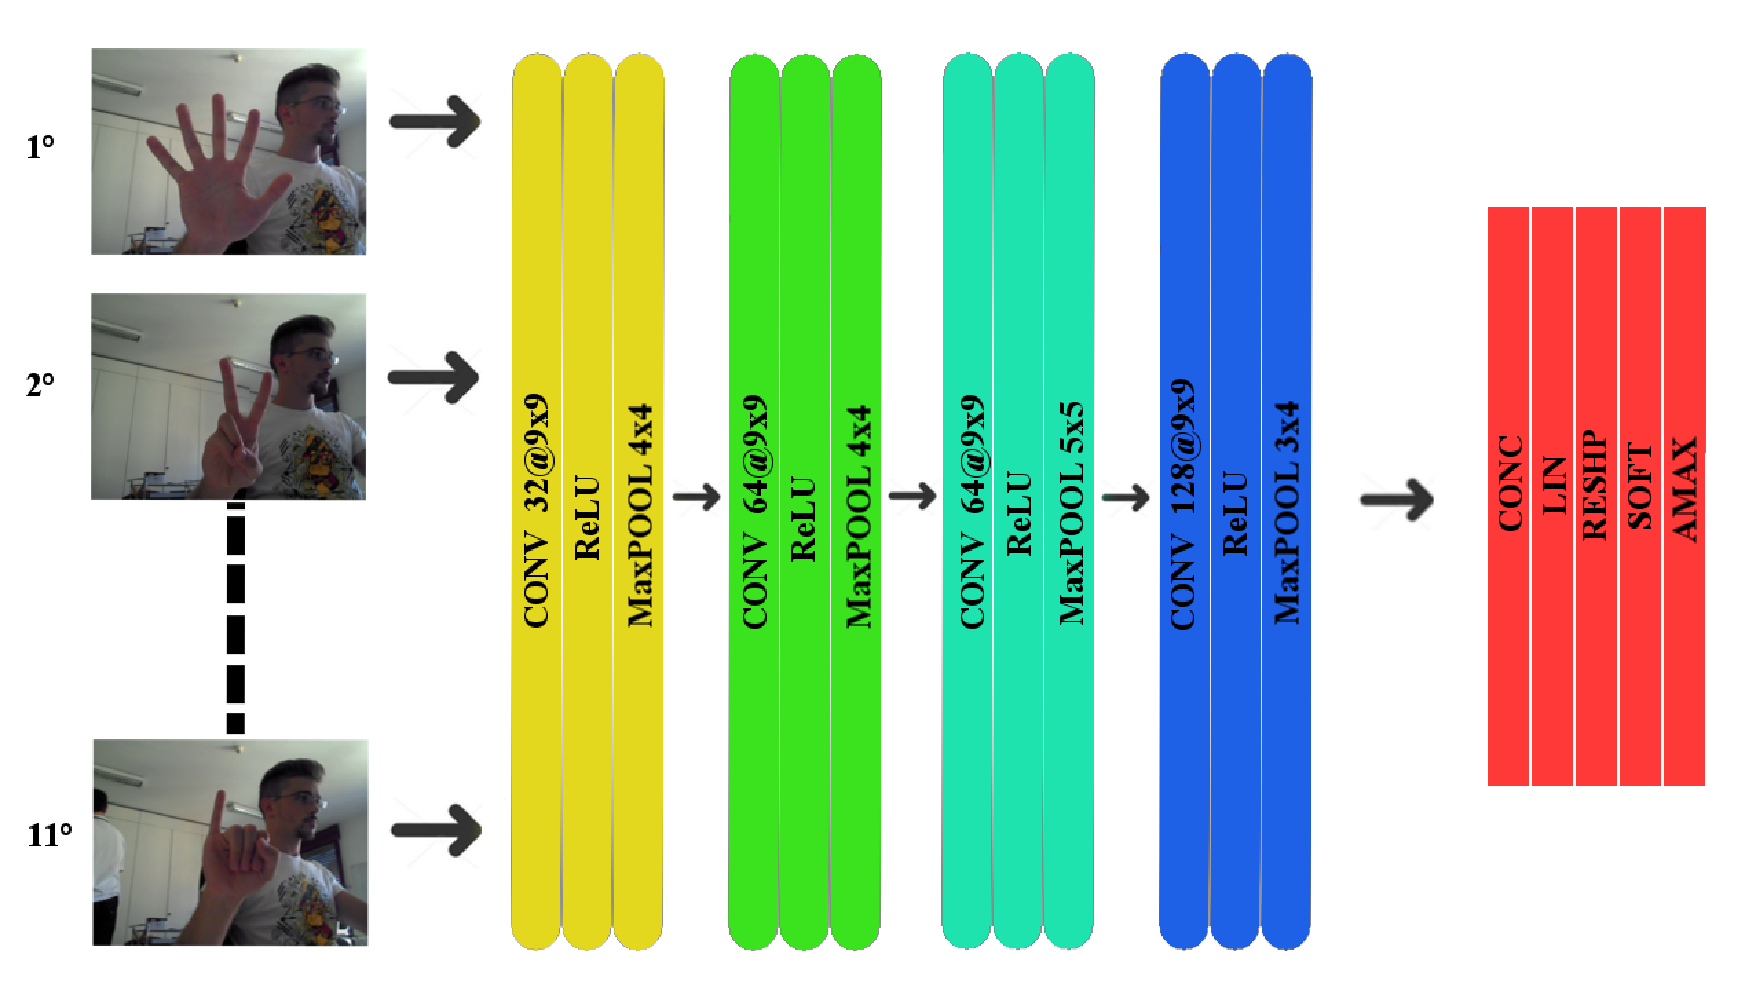
\includegraphics[width=%
1\textwidth]{figures/LivelliConv}
\caption[Struttura della rete.]{Si hanno in ingresso le immagini, elaborate precedentemente, relative agli unidici gesti. Esse passano attraverso quattro layer di convoluzione, in cui sono applicate le funzioni di filtraggio, di normalizzazione e di pooling. Infine, tramite le ultime funzioni vengono classificate. 
\label{fig:strutturarete}}
\end{figure}

I livelli vengono collegati secondo configurazioni diverse in base all'approccio seguito. In questo progetto di ricerca sono proposti cinque approcci differenti. In tal modo è stato possibile avere confronti tra di essi per un risultato finale più completo.\\

\section{Approcci proposti}
Gli approcci si differenziano in base ai dati di input utilizzati per ognuno di essi e qundi, di conseguenza, alle varie configurazioni della rete e del numero di canali. La Tabella \textbf{\ref{Approcci}} schematizza i vari approcci secondo i tipi di dati di input usati. 

% h means here: Place the figure in the text where the figure environment is written, if there is enough room left on the page
% t means top: Place it at the top of a page.
% b means bottom: Place it at the bottom of a page.
% p means page: Place it on a page containing only floats, such as figures and tables.

\begin{table}[htbp]
  \centering
  \caption{Tabella Approcci}\label{Approcci}
  \medskip
\begin{tabular}{cccccccc}
\toprule
& \multicolumn{7}{c}{\textbf{Approcci}} \\
\textbf{Dati di Input} &  \textbf{1°} &  \textbf{1°} &  \textbf{1°}  &  \textbf{2°}  &  \textbf{3°}  &  \textbf{4°}  &  \textbf{5°}  \\
\midrule
\rowcolor{gray!45}
Depth & \checkmark & & & \checkmark & & \checkmark & \checkmark \\
Conf & & \checkmark & & \checkmark & & \checkmark & \checkmark \\
\rowcolor{gray!45}
Color - R & & & &  & \checkmark  & \checkmark & \checkmark \\
Color - G & & & &  & \checkmark  & \checkmark & \checkmark \\
\rowcolor{gray!45}
Color - B & & & &  & \checkmark  & \checkmark & \checkmark \\
Grey-Scale & & & \checkmark & \checkmark & & & \\
\bottomrule
\end{tabular}
\end{table}


\subsection{Approccio unidimensionale 1 canale }
Il 1° approccio e più semplice, viene ulteriormente suddiviso in tre parti in base ai dati di input scelti ed è caratterizzato da un unico canale unidimensionale. In questo approccio è applicato lo studio su dati di profondità (DEPTH), dati di confidenza (CONF) proporzionali all'ampiezza del segnale di uscita ToF del sensore di profondità e dati basati sul colore in scala di grigi (GREYSCALE). Ogni sottoapproccio viene eseguito in modo separato, cioè con cicli distinti di training/testing della rete.
Quindi vengono riportati i risultati per ognuna delle tre categorie in modo indipendente una dell'altra.

\subsection{Approccio unidimensionale 3 canali: Depth, Conf, Greyscale}
Il 2° approccio utilizza le stesse tipologie di dati del primo. Però, invece di avere un unico canale e di fare uno studio indipendente per ogni classe di dati, sono creati 3 canali unidimensionali tramite un'architettura multi-branch (multicanale). Viene assegnato un canale per ogni tipologia di dati DEPTH, CONF e GREYSCALE. L'input della rete è la combinazione dei 3 canali in un unico ciclo di training e testing. Riguardo questo tipo di architettura si rimanda all'articolo \cite{Zhang2018DeepNN} e alle sua bibliografia per una spiegazione dettagliata.

\subsection{Approccio unidimensionale 3 canali: Color RGB}
Ha la stessa struttura del secondo approccio. L'unica differenza è la tipologia di dati di input scelta. Ora lo studio è fatto su dati basati sul colore che seguono il modello RGB. Quindi è assegnato un canale unidimensionale per ciascuno dei tre colori ( Rosso-Verde-Blu). Le restanti caratteristiche di questo 3° approccio coincidono con l'approccio precedente.

\subsection{Approccio unidimensionale 5 canali: Depth, Conf, Color RGB}
Composto da una combinazione del secondo e del terzo, in quanto il numero di canali unidimensionali è aumentato a cinque e sono assegnati ad essi i dati di input di profondità (DEPTH), di confidenza (CONF) e di colore RGB (quindi 3 canali unidimensionali per il colore). Anch'esso crea una combinazione di questi canali come input per cercare di migliorare l'apprendimento basandosi su più fattori contemporaneamente.

\subsection{Approccio pentadimensionale 1 canale: Depth, Conf, Color RGB}
Infine l'ultimo approccio riprende quasi tutti gli aspetti del quarto ma con una eccezione. Invece di avere canali unidimensionali per ognuna delle cinque tipologie di dati (DEPTH, CONF, RGB), si utilizza un unico canale multi-dimensionale (penta-dimensionale). Questo metodo comporta delle differenze sui dati i quali vengono combinati dall'inizio (rispetto al 4° approccio in cui questo avviene nell'ultimo layer). Quindi gli algoritmi che vengono utilizzati non saranno più eseguiti in modo distinto per ogni canale per poi unire i risultati successivamente, ma saranno applicati a tutti i dati insieme in quanto essi sono raggruppati in un canale unico. Non è scontato che questo approccio migliori l'apprendimento rispetto a quello precedente. Sicuramente si potranno avere situazioni in cui è preferibile usare questo approccio ed altri in cui funzionerà meglio un approccio unidimensionale.\\

In dettaglio, il primo approccio è quello base che utilizza un unico canale unidimensionale. In questo caso la rete neurale è anch'essa unidimensionale composta da quattro blocchi principali ciascuno contenente tre strati (Figura \textbf{\ref{fig:strutturarete}}). Ogni blocco è composto da uno strato convoluzionale (CONV) seguito da una funzione di normalizzazione (ReLU) e completato da un layer Max-Pooling finale (MaxPOOL) mentre il classificatore pixel-wise Softmax è applicato sopra l'ultimo strato convoluzionale.
Per ridurre il tempo di calcolo, le immagini di input hanno una risoluzione ridotta di 320x240. Gli strati convoluzionali hanno rispettivamente 32, 64, 64, 128 filtri dal primo al quarto, tutti di dimensione 9x9 pixel, mentre il classificatore Softmax ha una
matrice di peso della dimensione 128x11 e nessun bias.
Viene applicata, la normalizzazione del contrasto locale a ciascun canale di input indipendentemente, consentendo ai pesi del filtro nel primo strato convoluzionale di convergere più velocemente.
Nel primo approccio non viene usata la funzione di concatenazione (CONC).
Negli approcci successivi la costruzione della rete neurale è simile ma si hanno più canali di input contemporaneamente e quindi un'architettura multi-branch. Per ognuno di essi, la rete ha i quattro blocchi principali con tutte le relative funzione spiegate sopra.
In questi casi viene poi applicata la funzione di concatenazione e restano invariate le funzioni successive.
L'eccezione si trova nel quinto approccio in cui si torna a lavorare con un solo canale, ma stavolta multi-dimensionale.
Viene mostrato un pezzo del codice per l'assegnazione del vettore penta-dimensionale contenente i dati di DEPTH, CONF, RGB.
La composizione della rete neurale è invariata rispetto ai casi del primo approccio. \\

\textbf{Codice:} Assegnazione del vettore di input pentadimensionale nel 5° approccio.
\begin{python}
inpt=np.zeros(shape=(5,240,320),dtype=np.float32)

inpt1=pc.resize(depth[0,:,:],(240, 320),'linear').astype('float32')
inpt1=pc.normalize(inpt1,'local',1.8,1.8)
inpt[0,:,:]=inpt1

inpt2=pc.resize(conf[0,:,:],(240, 320),'linear').astype('float32')
inpt2=pc.normalize(inpt2, 'local',1.8,1.8)
inpt2=np.expand_dims(inpt2, axis=0)
inpt[1,:,:]= inpt2
        
img=pc.resize(img[:,:,:],(240,320,3),'linear').astype('float32')
inpt3=pc.normalize(img,'local',1.8,1.8)
        
inpt[2,:,:]=inpt3[:,:,2]
inpt[3,:,:]=inpt3[:,:,1]
inpt[4,:,:]=inpt3[:,:,0]
\end{python}


\begin{comment}
\begin{figure}
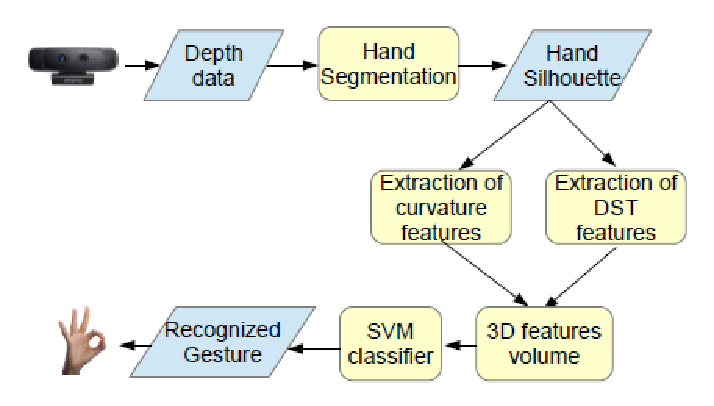
\includegraphics[width=%
0.8\textwidth]{figures/fig12}
\caption[Struttura algoritmo gesture.]{Figura rappresentativa .
\label{fig:myInlineFigure}}
\end{figure}
\end{comment}






